\documentclass{standalone}
\usepackage{tikz}
\usetikzlibrary{patterns, positioning}
\usepackage[sfdefault]{ClearSans} %% option 'sfdefault' activates Clear Sans as the default text font
\usepackage[T1]{fontenc}

\begin{document}
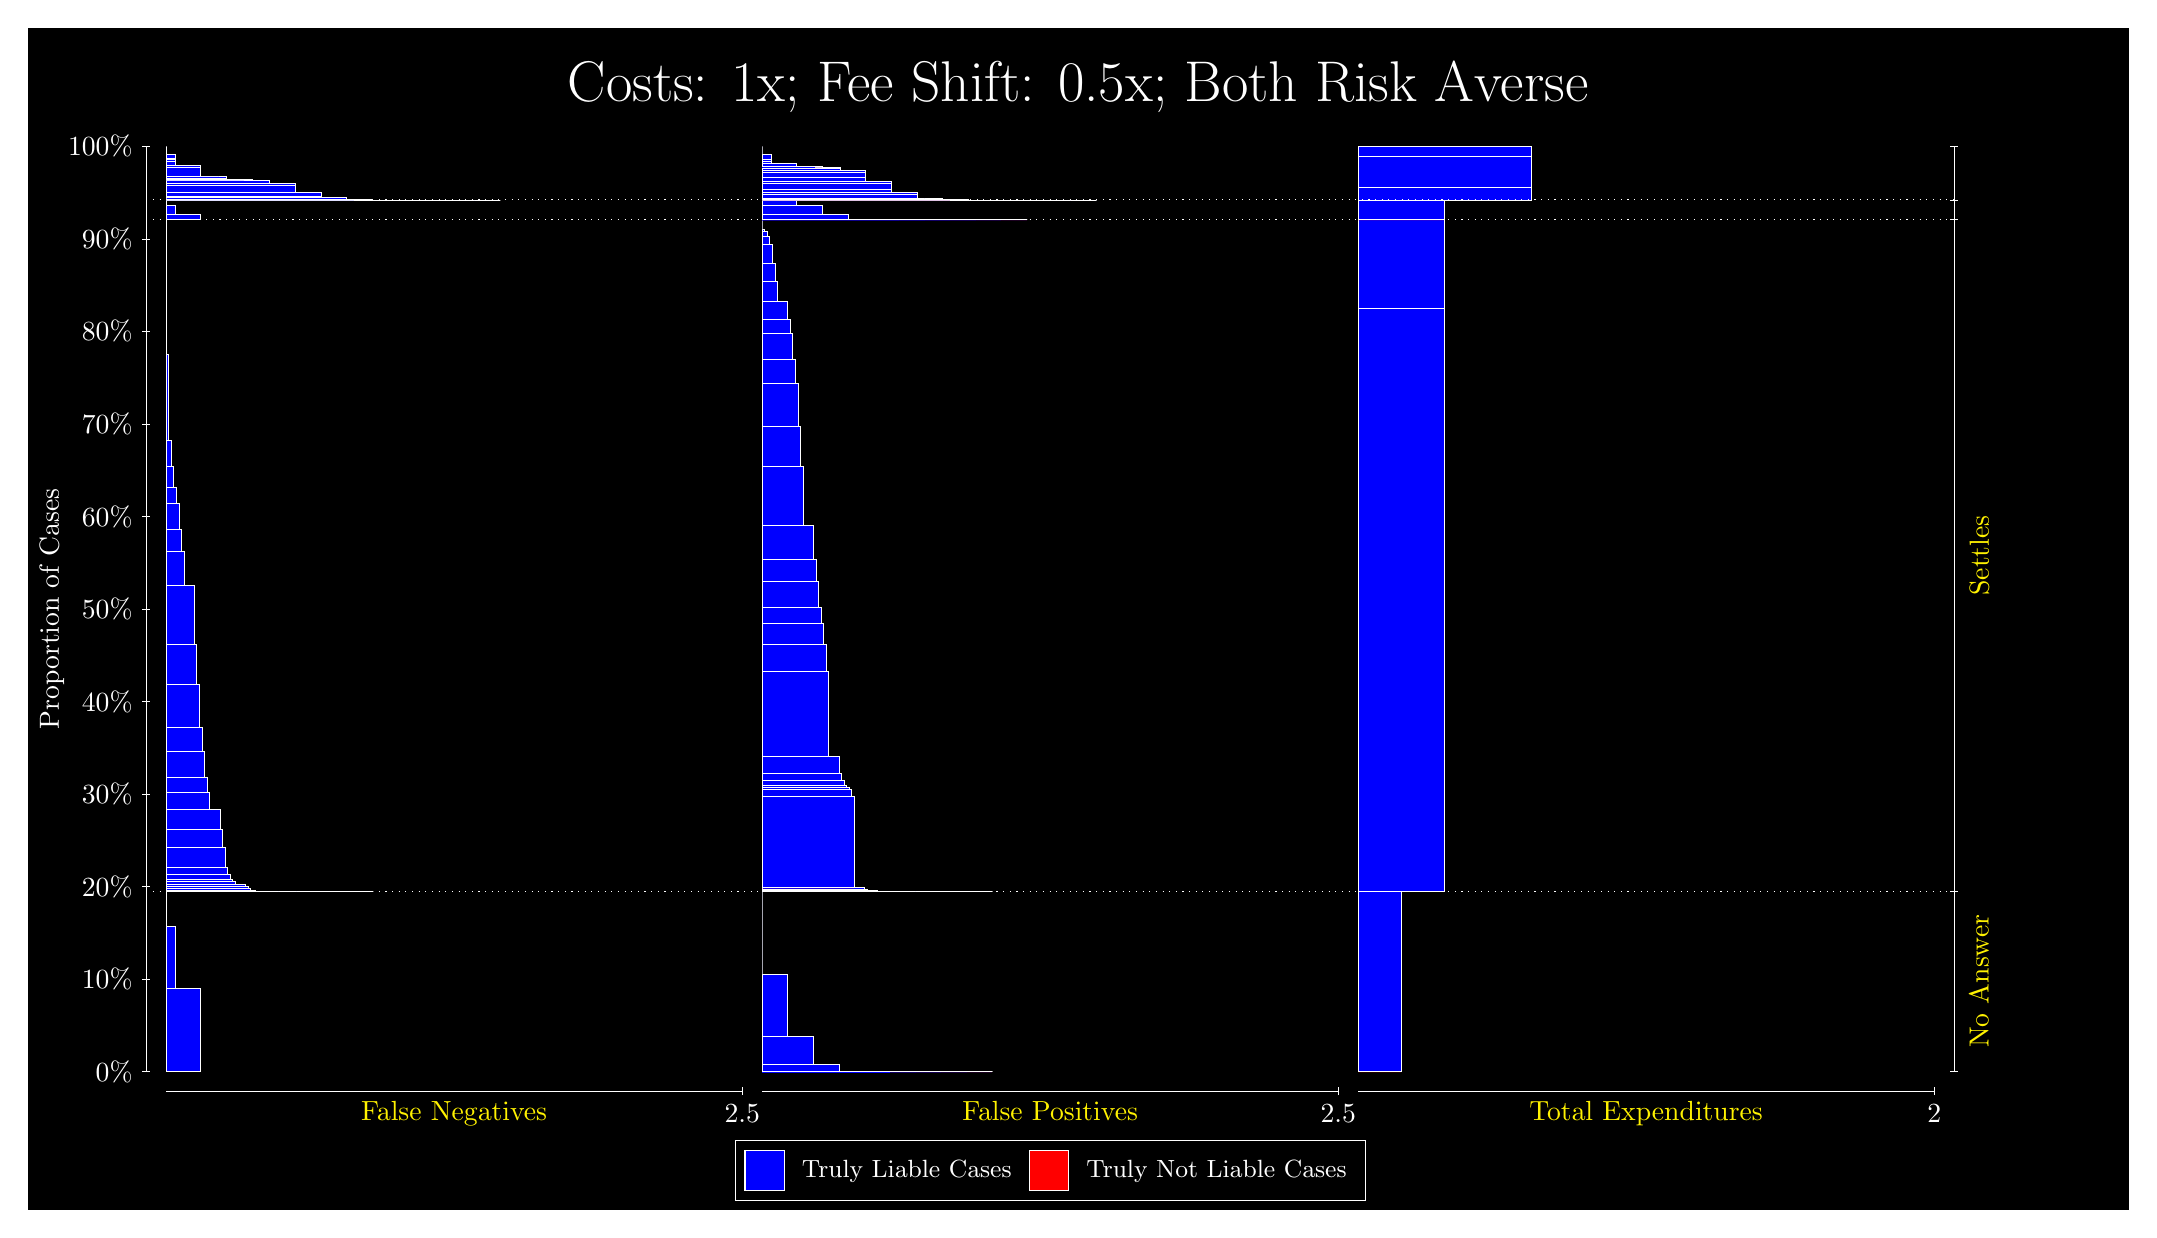
\begin{tikzpicture}
\draw[fill=black] (0,0) rectangle (26.667,15);
\draw[text=white] (0,13.5) rectangle (26.667,15) node[midway] {\huge Costs: 1x; Fee Shift: 0.5x; Both Risk Averse};
\draw[white, very thin] (1.5,1.75) -- (1.5,13.5);
\node[rotate=90, text=white, anchor=center] at (0.3, 7.625) {Proportion of Cases};
\draw[white, very thin] (1.45,1.75) -- (1.55,1.75);
\node[text=white, anchor=east] at (1.45, 1.75) {0\%};
\draw[white, very thin] (1.45,2.925) -- (1.55,2.925);
\node[text=white, anchor=east] at (1.45, 2.925) {10\%};
\draw[white, very thin] (1.45,4.1) -- (1.55,4.1);
\node[text=white, anchor=east] at (1.45, 4.1) {20\%};
\draw[white, very thin] (1.45,5.275) -- (1.55,5.275);
\node[text=white, anchor=east] at (1.45, 5.275) {30\%};
\draw[white, very thin] (1.45,6.45) -- (1.55,6.45);
\node[text=white, anchor=east] at (1.45, 6.45) {40\%};
\draw[white, very thin] (1.45,7.625) -- (1.55,7.625);
\node[text=white, anchor=east] at (1.45, 7.625) {50\%};
\draw[white, very thin] (1.45,8.8) -- (1.55,8.8);
\node[text=white, anchor=east] at (1.45, 8.8) {60\%};
\draw[white, very thin] (1.45,9.975) -- (1.55,9.975);
\node[text=white, anchor=east] at (1.45, 9.975) {70\%};
\draw[white, very thin] (1.45,11.15) -- (1.55,11.15);
\node[text=white, anchor=east] at (1.45, 11.15) {80\%};
\draw[white, very thin] (1.45,12.325) -- (1.55,12.325);
\node[text=white, anchor=east] at (1.45, 12.325) {90\%};
\draw[white, very thin] (1.45,13.5) -- (1.55,13.5);
\node[text=white, anchor=east] at (1.45, 13.5) {100\%};

\draw[white, very thin] (24.457,1.75) -- (24.457,13.5);
\draw[white, very thin] (24.407,1.75) -- (24.507,1.75);
\node[anchor=west] at (24.407, 1.75) {};
\draw[white, very thin] (24.407,4.0413) -- (24.507,4.0413);
\node[anchor=west] at (24.407, 4.0413) {};
\draw[white, very thin] (24.407,12.569) -- (24.507,12.569);
\node[anchor=west] at (24.407, 12.569) {};
\draw[white, very thin] (24.407,12.819) -- (24.507,12.819);
\node[anchor=west] at (24.407, 12.819) {};
\draw[white, very thin] (24.407,13.5) -- (24.507,13.5);
\node[anchor=west] at (24.407, 13.5) {};

\draw[white, very thin, fill=blue] (1.75,1.75) rectangle (2.1891,2.8115);
\draw[white, very thin, fill=blue] (1.75,2.8115) rectangle (1.8638,3.598);
\draw[white, very thin, fill=red] (1.75,3.598) rectangle (1.75,3.598);
\draw[white, very thin, fill=blue] (1.75,3.598) rectangle (1.75,4.0413);
\draw[white, very thin, fill=blue] (1.75,4.0413) rectangle (4.3848,4.0413);
\draw[white, very thin, fill=blue] (1.75,4.0413) rectangle (4.092,4.0413);
\draw[white, very thin, fill=blue] (1.75,4.0413) rectangle (4.0595,4.0413);
\draw[white, very thin, fill=blue] (1.75,4.0413) rectangle (3.7993,4.0413);
\draw[white, very thin, fill=blue] (1.75,4.0413) rectangle (3.7668,4.0413);
\draw[white, very thin, fill=blue] (1.75,4.0413) rectangle (3.7342,4.0413);
\draw[white, very thin, fill=blue] (1.75,4.0413) rectangle (3.5065,4.0413);
\draw[white, very thin, fill=blue] (1.75,4.0413) rectangle (3.474,4.0413);
\draw[white, very thin, fill=blue] (1.75,4.0413) rectangle (3.4415,4.0413);
\draw[white, very thin, fill=blue] (1.75,4.0413) rectangle (3.4089,4.0413);
\draw[white, very thin, fill=blue] (1.75,4.0413) rectangle (3.2138,4.0414);
\draw[white, very thin, fill=blue] (1.75,4.0414) rectangle (3.1812,4.0414);
\draw[white, very thin, fill=blue] (1.75,4.0414) rectangle (3.1487,4.0419);
\draw[white, very thin, fill=blue] (1.75,4.0419) rectangle (3.1162,4.0424);
\draw[white, very thin, fill=blue] (1.75,4.0424) rectangle (3.0837,4.0429);
\draw[white, very thin, fill=blue] (1.75,4.0429) rectangle (2.921,4.0439);
\draw[white, very thin, fill=blue] (1.75,4.0439) rectangle (2.8885,4.0469);
\draw[white, very thin, fill=blue] (1.75,4.0469) rectangle (2.856,4.0519);
\draw[white, very thin, fill=blue] (1.75,4.0519) rectangle (2.8234,4.0773);
\draw[white, very thin, fill=blue] (1.75,4.0773) rectangle (2.7909,4.101);
\draw[white, very thin, fill=blue] (1.75,4.101) rectangle (2.7584,4.1252);
\draw[white, very thin, fill=blue] (1.75,4.1252) rectangle (2.6283,4.1668);
\draw[white, very thin, fill=blue] (1.75,4.1668) rectangle (2.5957,4.1915);
\draw[white, very thin, fill=blue] (1.75,4.1915) rectangle (2.5632,4.2584);
\draw[white, very thin, fill=blue] (1.75,4.2584) rectangle (2.5307,4.3489);
\draw[white, very thin, fill=blue] (1.75,4.3489) rectangle (2.4982,4.6008);
\draw[white, very thin, fill=blue] (1.75,4.6008) rectangle (2.4656,4.8273);
\draw[white, very thin, fill=blue] (1.75,4.8273) rectangle (2.4331,5.0778);
\draw[white, very thin, fill=blue] (1.75,5.0778) rectangle (2.303,5.3013);
\draw[white, very thin, fill=blue] (1.75,5.3013) rectangle (2.2705,5.4809);
\draw[white, very thin, fill=blue] (1.75,5.4809) rectangle (2.2379,5.8118);
\draw[white, very thin, fill=blue] (1.75,5.8118) rectangle (2.2054,6.1165);
\draw[white, very thin, fill=blue] (1.75,6.1165) rectangle (2.1729,6.6626);
\draw[white, very thin, fill=blue] (1.75,6.6626) rectangle (2.1403,7.1702);
\draw[white, very thin, fill=blue] (1.75,7.1702) rectangle (2.1078,7.926);
\draw[white, very thin, fill=blue] (1.75,7.926) rectangle (1.9777,8.3542);
\draw[white, very thin, fill=blue] (1.75,8.3542) rectangle (1.9452,8.6354);
\draw[white, very thin, fill=blue] (1.75,8.6354) rectangle (1.9126,8.966);
\draw[white, very thin, fill=blue] (1.75,8.966) rectangle (1.8801,9.1676);
\draw[white, very thin, fill=blue] (1.75,9.1676) rectangle (1.8476,9.4388);
\draw[white, very thin, fill=blue] (1.75,9.4388) rectangle (1.8151,9.7722);
\draw[white, very thin, fill=blue] (1.75,9.7722) rectangle (1.7825,10.856);
\draw[white, very thin, fill=red] (1.75,10.856) rectangle (1.75,10.856);
\draw[white, very thin, fill=blue] (1.75,10.856) rectangle (1.75,12.569);
\draw[white, very thin, fill=blue] (1.75,12.569) rectangle (2.1891,12.635);
\draw[white, very thin, fill=blue] (1.75,12.635) rectangle (1.8638,12.749);
\draw[white, very thin, fill=red] (1.75,12.749) rectangle (1.75,12.749);
\draw[white, very thin, fill=blue] (1.75,12.749) rectangle (1.75,12.819);
\draw[white, very thin, fill=blue] (1.75,12.819) rectangle (5.9949,12.819);
\draw[white, very thin, fill=blue] (1.75,12.819) rectangle (5.6697,12.819);
\draw[white, very thin, fill=blue] (1.75,12.819) rectangle (5.3444,12.819);
\draw[white, very thin, fill=blue] (1.75,12.819) rectangle (5.3444,12.819);
\draw[white, very thin, fill=blue] (1.75,12.819) rectangle (5.0191,12.819);
\draw[white, very thin, fill=blue] (1.75,12.819) rectangle (4.6938,12.82);
\draw[white, very thin, fill=blue] (1.75,12.82) rectangle (4.3685,12.824);
\draw[white, very thin, fill=blue] (1.75,12.824) rectangle (4.1408,12.824);
\draw[white, very thin, fill=blue] (1.75,12.824) rectangle (4.0432,12.833);
\draw[white, very thin, fill=blue] (1.75,12.833) rectangle (4.0432,12.848);
\draw[white, very thin, fill=blue] (1.75,12.848) rectangle (3.8155,12.848);
\draw[white, very thin, fill=blue] (1.75,12.848) rectangle (3.8155,12.848);
\draw[white, very thin, fill=blue] (1.75,12.848) rectangle (3.718,12.863);
\draw[white, very thin, fill=blue] (1.75,12.863) rectangle (3.718,12.922);
\draw[white, very thin, fill=blue] (1.75,12.922) rectangle (3.4903,12.922);
\draw[white, very thin, fill=blue] (1.75,12.922) rectangle (3.3927,13.005);
\draw[white, very thin, fill=blue] (1.75,13.005) rectangle (3.3927,13.029);
\draw[white, very thin, fill=blue] (1.75,13.029) rectangle (3.165,13.029);
\draw[white, very thin, fill=blue] (1.75,13.029) rectangle (3.165,13.029);
\draw[white, very thin, fill=blue] (1.75,13.029) rectangle (3.0674,13.075);
\draw[white, very thin, fill=blue] (1.75,13.075) rectangle (2.8397,13.078);
\draw[white, very thin, fill=blue] (1.75,13.078) rectangle (2.7421,13.078);
\draw[white, very thin, fill=blue] (1.75,13.078) rectangle (2.7421,13.081);
\draw[white, very thin, fill=blue] (1.75,13.081) rectangle (2.7421,13.082);
\draw[white, very thin, fill=blue] (1.75,13.082) rectangle (2.5144,13.098);
\draw[white, very thin, fill=blue] (1.75,13.098) rectangle (2.5144,13.123);
\draw[white, very thin, fill=blue] (1.75,13.123) rectangle (2.4168,13.123);
\draw[white, very thin, fill=blue] (1.75,13.123) rectangle (2.4168,13.123);
\draw[white, very thin, fill=blue] (1.75,13.123) rectangle (2.1891,13.229);
\draw[white, very thin, fill=blue] (1.75,13.229) rectangle (2.1891,13.259);
\draw[white, very thin, fill=blue] (1.75,13.259) rectangle (2.0915,13.259);
\draw[white, very thin, fill=blue] (1.75,13.259) rectangle (2.0915,13.259);
\draw[white, very thin, fill=blue] (1.75,13.259) rectangle (1.8638,13.306);
\draw[white, very thin, fill=blue] (1.75,13.306) rectangle (1.8638,13.33);
\draw[white, very thin, fill=blue] (1.75,13.33) rectangle (1.8638,13.342);
\draw[white, very thin, fill=blue] (1.75,13.342) rectangle (1.8638,13.4);
\draw[white, very thin, fill=blue] (1.75,13.4) rectangle (1.7663,13.4);
\draw[white, very thin, fill=blue] (1.75,13.4) rectangle (1.7663,13.4);
\draw[white, very thin, fill=red] (1.75,13.4) rectangle (1.75,13.4);
\draw[white, very thin, fill=blue] (1.75,13.4) rectangle (1.75,13.5);
\draw[white, very thin, fill=red] (9.3189,1.75) rectangle (12.246,1.75);
\draw[white, very thin, fill=blue] (9.3189,1.75) rectangle (12.246,1.75);
\draw[white, very thin, fill=blue] (9.3189,1.75) rectangle (11.921,1.75);
\draw[white, very thin, fill=blue] (9.3189,1.75) rectangle (11.596,1.75);
\draw[white, very thin, fill=blue] (9.3189,1.75) rectangle (11.271,1.75);
\draw[white, very thin, fill=blue] (9.3189,1.75) rectangle (10.945,1.7503);
\draw[white, very thin, fill=blue] (9.3189,1.7503) rectangle (10.62,1.7576);
\draw[white, very thin, fill=blue] (9.3189,1.7576) rectangle (10.295,1.8358);
\draw[white, very thin, fill=blue] (9.3189,1.8358) rectangle (9.9694,2.1933);
\draw[white, very thin, fill=blue] (9.3189,2.1933) rectangle (9.6442,2.9798);
\draw[white, very thin, fill=blue] (9.3189,2.9798) rectangle (9.3189,4.0413);
\draw[white, very thin, fill=red] (9.3189,4.0413) rectangle (12.246,4.0413);
\draw[white, very thin, fill=blue] (9.3189,4.0413) rectangle (12.246,4.0413);
\draw[white, very thin, fill=red] (9.3189,4.0413) rectangle (11.954,4.0413);
\draw[white, very thin, fill=blue] (9.3189,4.0413) rectangle (11.954,4.0413);
\draw[white, very thin, fill=blue] (9.3189,4.0413) rectangle (11.921,4.0413);
\draw[white, very thin, fill=red] (9.3189,4.0413) rectangle (11.661,4.0413);
\draw[white, very thin, fill=blue] (9.3189,4.0413) rectangle (11.661,4.0413);
\draw[white, very thin, fill=blue] (9.3189,4.0413) rectangle (11.628,4.0413);
\draw[white, very thin, fill=blue] (9.3189,4.0413) rectangle (11.596,4.0413);
\draw[white, very thin, fill=red] (9.3189,4.0413) rectangle (11.368,4.0413);
\draw[white, very thin, fill=blue] (9.3189,4.0413) rectangle (11.368,4.0413);
\draw[white, very thin, fill=blue] (9.3189,4.0413) rectangle (11.336,4.0413);
\draw[white, very thin, fill=blue] (9.3189,4.0413) rectangle (11.303,4.0413);
\draw[white, very thin, fill=blue] (9.3189,4.0413) rectangle (11.271,4.0413);
\draw[white, very thin, fill=red] (9.3189,4.0413) rectangle (11.075,4.0413);
\draw[white, very thin, fill=blue] (9.3189,4.0413) rectangle (11.075,4.0413);
\draw[white, very thin, fill=blue] (9.3189,4.0413) rectangle (11.043,4.0413);
\draw[white, very thin, fill=blue] (9.3189,4.0413) rectangle (11.01,4.0413);
\draw[white, very thin, fill=blue] (9.3189,4.0413) rectangle (10.978,4.0414);
\draw[white, very thin, fill=blue] (9.3189,4.0414) rectangle (10.945,4.0419);
\draw[white, very thin, fill=red] (9.3189,4.0419) rectangle (10.783,4.0419);
\draw[white, very thin, fill=blue] (9.3189,4.0419) rectangle (10.783,4.0524);
\draw[white, very thin, fill=blue] (9.3189,4.0524) rectangle (10.75,4.0533);
\draw[white, very thin, fill=blue] (9.3189,4.0533) rectangle (10.718,4.054);
\draw[white, very thin, fill=blue] (9.3189,4.054) rectangle (10.685,4.0566);
\draw[white, very thin, fill=blue] (9.3189,4.0566) rectangle (10.653,4.0614);
\draw[white, very thin, fill=blue] (9.3189,4.0614) rectangle (10.62,4.0846);
\draw[white, very thin, fill=red] (9.3189,4.0846) rectangle (10.49,4.0846);
\draw[white, very thin, fill=blue] (9.3189,4.0846) rectangle (10.49,5.2486);
\draw[white, very thin, fill=blue] (9.3189,5.2486) rectangle (10.457,5.3319);
\draw[white, very thin, fill=blue] (9.3189,5.3319) rectangle (10.425,5.3624);
\draw[white, very thin, fill=blue] (9.3189,5.3624) rectangle (10.392,5.389);
\draw[white, very thin, fill=blue] (9.3189,5.389) rectangle (10.36,5.4551);
\draw[white, very thin, fill=blue] (9.3189,5.4551) rectangle (10.327,5.541);
\draw[white, very thin, fill=blue] (9.3189,5.541) rectangle (10.295,5.754);
\draw[white, very thin, fill=blue] (9.3189,5.754) rectangle (10.165,6.8377);
\draw[white, very thin, fill=blue] (9.3189,6.8377) rectangle (10.132,7.1711);
\draw[white, very thin, fill=blue] (9.3189,7.1711) rectangle (10.1,7.4423);
\draw[white, very thin, fill=blue] (9.3189,7.4423) rectangle (10.067,7.6439);
\draw[white, very thin, fill=blue] (9.3189,7.6439) rectangle (10.034,7.9745);
\draw[white, very thin, fill=blue] (9.3189,7.9745) rectangle (10.002,8.2557);
\draw[white, very thin, fill=blue] (9.3189,8.2557) rectangle (9.9694,8.6839);
\draw[white, very thin, fill=blue] (9.3189,8.6839) rectangle (9.8393,9.4397);
\draw[white, very thin, fill=blue] (9.3189,9.4397) rectangle (9.8068,9.9473);
\draw[white, very thin, fill=blue] (9.3189,9.9473) rectangle (9.7743,10.493);
\draw[white, very thin, fill=blue] (9.3189,10.493) rectangle (9.7417,10.798);
\draw[white, very thin, fill=blue] (9.3189,10.798) rectangle (9.7092,11.129);
\draw[white, very thin, fill=blue] (9.3189,11.129) rectangle (9.6767,11.309);
\draw[white, very thin, fill=blue] (9.3189,11.309) rectangle (9.6442,11.532);
\draw[white, very thin, fill=blue] (9.3189,11.532) rectangle (9.514,11.783);
\draw[white, very thin, fill=blue] (9.3189,11.783) rectangle (9.4815,12.009);
\draw[white, very thin, fill=blue] (9.3189,12.009) rectangle (9.449,12.261);
\draw[white, very thin, fill=blue] (9.3189,12.261) rectangle (9.4165,12.352);
\draw[white, very thin, fill=blue] (9.3189,12.352) rectangle (9.3839,12.418);
\draw[white, very thin, fill=blue] (9.3189,12.418) rectangle (9.3514,12.443);
\draw[white, very thin, fill=blue] (9.3189,12.443) rectangle (9.3189,12.569);
\draw[white, very thin, fill=red] (9.3189,12.569) rectangle (12.686,12.569);
\draw[white, very thin, fill=blue] (9.3189,12.569) rectangle (12.686,12.569);
\draw[white, very thin, fill=blue] (9.3189,12.569) rectangle (12.36,12.569);
\draw[white, very thin, fill=blue] (9.3189,12.569) rectangle (12.035,12.569);
\draw[white, very thin, fill=blue] (9.3189,12.569) rectangle (11.71,12.569);
\draw[white, very thin, fill=blue] (9.3189,12.569) rectangle (11.384,12.569);
\draw[white, very thin, fill=blue] (9.3189,12.569) rectangle (11.059,12.569);
\draw[white, very thin, fill=blue] (9.3189,12.569) rectangle (10.734,12.577);
\draw[white, very thin, fill=blue] (9.3189,12.577) rectangle (10.409,12.639);
\draw[white, very thin, fill=blue] (9.3189,12.639) rectangle (10.083,12.752);
\draw[white, very thin, fill=blue] (9.3189,12.752) rectangle (9.758,12.819);
\draw[white, very thin, fill=red] (9.3189,12.819) rectangle (13.564,12.819);
\draw[white, very thin, fill=blue] (9.3189,12.819) rectangle (13.564,12.819);
\draw[white, very thin, fill=red] (9.3189,12.819) rectangle (13.239,12.819);
\draw[white, very thin, fill=blue] (9.3189,12.819) rectangle (13.239,12.819);
\draw[white, very thin, fill=red] (9.3189,12.819) rectangle (12.913,12.819);
\draw[white, very thin, fill=blue] (9.3189,12.819) rectangle (12.913,12.819);
\draw[white, very thin, fill=blue] (9.3189,12.819) rectangle (12.913,12.819);
\draw[white, very thin, fill=red] (9.3189,12.819) rectangle (12.588,12.819);
\draw[white, very thin, fill=blue] (9.3189,12.819) rectangle (12.588,12.819);
\draw[white, very thin, fill=red] (9.3189,12.819) rectangle (12.263,12.819);
\draw[white, very thin, fill=blue] (9.3189,12.819) rectangle (12.263,12.819);
\draw[white, very thin, fill=red] (9.3189,12.819) rectangle (12.035,12.819);
\draw[white, very thin, fill=blue] (9.3189,12.819) rectangle (12.035,12.819);
\draw[white, very thin, fill=blue] (9.3189,12.819) rectangle (11.937,12.82);
\draw[white, very thin, fill=blue] (9.3189,12.82) rectangle (11.937,12.821);
\draw[white, very thin, fill=red] (9.3189,12.821) rectangle (11.937,12.821);
\draw[white, very thin, fill=blue] (9.3189,12.821) rectangle (11.937,12.823);
\draw[white, very thin, fill=red] (9.3189,12.823) rectangle (11.71,12.823);
\draw[white, very thin, fill=blue] (9.3189,12.823) rectangle (11.71,12.823);
\draw[white, very thin, fill=blue] (9.3189,12.823) rectangle (11.612,12.832);
\draw[white, very thin, fill=blue] (9.3189,12.832) rectangle (11.612,12.839);
\draw[white, very thin, fill=red] (9.3189,12.839) rectangle (11.612,12.839);
\draw[white, very thin, fill=blue] (9.3189,12.839) rectangle (11.612,12.845);
\draw[white, very thin, fill=red] (9.3189,12.845) rectangle (11.384,12.845);
\draw[white, very thin, fill=blue] (9.3189,12.845) rectangle (11.384,12.845);
\draw[white, very thin, fill=blue] (9.3189,12.845) rectangle (11.384,12.845);
\draw[white, very thin, fill=blue] (9.3189,12.845) rectangle (11.287,12.886);
\draw[white, very thin, fill=blue] (9.3189,12.886) rectangle (11.287,12.918);
\draw[white, very thin, fill=blue] (9.3189,12.918) rectangle (11.287,12.919);
\draw[white, very thin, fill=blue] (9.3189,12.919) rectangle (11.059,12.919);
\draw[white, very thin, fill=red] (9.3189,12.919) rectangle (11.059,12.919);
\draw[white, very thin, fill=blue] (9.3189,12.919) rectangle (11.059,12.919);
\draw[white, very thin, fill=blue] (9.3189,12.919) rectangle (10.962,12.949);
\draw[white, very thin, fill=blue] (9.3189,12.949) rectangle (10.962,13.031);
\draw[white, very thin, fill=blue] (9.3189,13.031) rectangle (10.962,13.06);
\draw[white, very thin, fill=blue] (9.3189,13.06) rectangle (10.734,13.06);
\draw[white, very thin, fill=blue] (9.3189,13.06) rectangle (10.734,13.06);
\draw[white, very thin, fill=red] (9.3189,13.06) rectangle (10.734,13.06);
\draw[white, very thin, fill=blue] (9.3189,13.06) rectangle (10.734,13.06);
\draw[white, very thin, fill=blue] (9.3189,13.06) rectangle (10.636,13.113);
\draw[white, very thin, fill=blue] (9.3189,13.113) rectangle (10.636,13.167);
\draw[white, very thin, fill=blue] (9.3189,13.167) rectangle (10.636,13.196);
\draw[white, very thin, fill=blue] (9.3189,13.196) rectangle (10.409,13.196);
\draw[white, very thin, fill=red] (9.3189,13.196) rectangle (10.409,13.196);
\draw[white, very thin, fill=blue] (9.3189,13.196) rectangle (10.409,13.196);
\draw[white, very thin, fill=blue] (9.3189,13.196) rectangle (10.409,13.196);
\draw[white, very thin, fill=blue] (9.3189,13.196) rectangle (10.311,13.198);
\draw[white, very thin, fill=blue] (9.3189,13.198) rectangle (10.311,13.222);
\draw[white, very thin, fill=blue] (9.3189,13.222) rectangle (10.311,13.237);
\draw[white, very thin, fill=blue] (9.3189,13.237) rectangle (10.083,13.238);
\draw[white, very thin, fill=blue] (9.3189,13.238) rectangle (10.083,13.241);
\draw[white, very thin, fill=red] (9.3189,13.241) rectangle (10.083,13.241);
\draw[white, very thin, fill=blue] (9.3189,13.241) rectangle (10.083,13.241);
\draw[white, very thin, fill=blue] (9.3189,13.241) rectangle (9.9857,13.242);
\draw[white, very thin, fill=blue] (9.3189,13.242) rectangle (9.9857,13.243);
\draw[white, very thin, fill=blue] (9.3189,13.243) rectangle (9.9857,13.244);
\draw[white, very thin, fill=blue] (9.3189,13.244) rectangle (9.758,13.287);
\draw[white, very thin, fill=red] (9.3189,13.287) rectangle (9.758,13.287);
\draw[white, very thin, fill=blue] (9.3189,13.287) rectangle (9.758,13.287);
\draw[white, very thin, fill=blue] (9.3189,13.287) rectangle (9.758,13.29);
\draw[white, very thin, fill=blue] (9.3189,13.29) rectangle (9.6604,13.29);
\draw[white, very thin, fill=blue] (9.3189,13.29) rectangle (9.6604,13.29);
\draw[white, very thin, fill=blue] (9.3189,13.29) rectangle (9.4327,13.314);
\draw[white, very thin, fill=blue] (9.3189,13.314) rectangle (9.4327,13.339);
\draw[white, very thin, fill=blue] (9.3189,13.339) rectangle (9.4327,13.341);
\draw[white, very thin, fill=blue] (9.3189,13.341) rectangle (9.4327,13.397);
\draw[white, very thin, fill=blue] (9.3189,13.397) rectangle (9.3351,13.397);
\draw[white, very thin, fill=blue] (9.3189,13.397) rectangle (9.3351,13.397);
\draw[white, very thin, fill=blue] (9.3189,13.397) rectangle (9.3189,13.5);
\draw[white, very thin, fill=red] (16.888,1.75) rectangle (17.437,1.75);
\draw[white, very thin, fill=blue] (16.888,1.75) rectangle (17.437,4.0413);
\draw[white, very thin, fill=red] (16.888,4.0413) rectangle (17.986,4.0413);
\draw[white, very thin, fill=blue] (16.888,4.0413) rectangle (17.986,11.442);
\draw[white, very thin, fill=red] (16.888,11.442) rectangle (17.986,11.442);
\draw[white, very thin, fill=blue] (16.888,11.442) rectangle (17.986,12.569);
\draw[white, very thin, fill=red] (16.888,12.569) rectangle (17.986,12.569);
\draw[white, very thin, fill=blue] (16.888,12.569) rectangle (17.986,12.819);
\draw[white, very thin, fill=red] (16.888,12.819) rectangle (19.083,12.819);
\draw[white, very thin, fill=blue] (16.888,12.819) rectangle (19.083,12.986);
\draw[white, very thin, fill=red] (16.888,12.986) rectangle (19.083,12.986);
\draw[white, very thin, fill=blue] (16.888,12.986) rectangle (19.083,13.379);
\draw[white, very thin, fill=red] (16.888,13.379) rectangle (19.083,13.379);
\draw[white, very thin, fill=blue] (16.888,13.379) rectangle (19.083,13.5);
\draw[white, dotted] (1.5,4.0413) -- (24.457,4.0413);
\draw[white, dotted] (1.5,12.569) -- (24.457,12.569);
\draw[white, dotted] (1.5,12.819) -- (24.457,12.819);
\draw[white, very thin] (1.75,1.5) -- (9.0689,1.5);
\node[text=yellow, anchor=north] at (5.4094, 1.5) {False Negatives};
\draw[white, very thin] (9.0689,1.45) -- (9.0689,1.55);
\node[text=white, anchor=north] at (9.0689, 1.45) {2.5};

\draw[white, very thin] (9.3189,1.5) -- (16.638,1.5);
\node[text=yellow, anchor=north] at (12.978, 1.5) {False Positives};
\draw[white, very thin] (16.638,1.45) -- (16.638,1.55);
\node[text=white, anchor=north] at (16.638, 1.45) {2.5};

\draw[white, very thin] (16.888,1.5) -- (24.207,1.5);
\node[text=yellow, anchor=north] at (20.547, 1.5) {Total Expenditures};
\draw[white, very thin] (24.207,1.45) -- (24.207,1.55);
\node[text=white, anchor=north] at (24.207, 1.45) {2};

\node[text=yellow, centered, rotate=90] at (24.777, 2.8957) {No Answer};
\node[text=yellow, centered, rotate=90] at (24.777, 8.305) {Settles};



\draw (12.978300999999998,1.5) node[draw=none] (baseCoordinate) {};
\begin{scope}[align=center]
        \matrix[scale=0.5, draw=white, below=0.5cm of baseCoordinate, nodes={draw}, column sep=0.1cm]{
            \node[rectangle, draw, minimum width=0.5cm, minimum height=0.5cm, fill=blue] {}; &
            \node[draw=none, font=\small, text=white] (B) {Truly Liable Cases}; &
            \node[rectangle, draw, minimum width=0.5cm, minimum height=0.5cm, fill=red] {}; &
            \node[draw=none, font=\small, text=white] (B) {Truly Not Liable Cases}; \\
            };
\end{scope}

\end{tikzpicture}
\end{document}